\documentclass[11pt, a4paper]{article}

\usepackage[utf8]{inputenc} % comment when using lualatex
\usepackage[italian]{babel} % lingua e a-capo-sillabato
\usepackage{graphicx}
\usepackage[hidelinks]{hyperref} % link di pagina
\usepackage[bottom]{footmisc} % note appiccicate al fondo della pagina
\usepackage{float} % per posizionamento immagini
\usepackage{amsthm} % per ambienti stile teorema
\usepackage{tabularx} %tabelle
\usepackage[table]{xcolor} %colore caselle
\usepackage{enumitem} %additional commands for lists
\usepackage{fancyhdr}
\usepackage[font=footnotesize,labelfont=bf]{caption} % small caption font-size
\usepackage{afterpage} %fancy does not include page numbers by default

\fancyhf{}% Clear header/footer
\pagestyle{fancy}
\fancyfoot[C]{\thepage} %add page number
\fancyhead[C]{\footnotesize\textit{Documento:} D2 \hfill SleepCode \hfill \textit{Versione:} 1.0}
\renewcommand{\headrule}{{\color{red!70}\rule{\textwidth}{2pt}}}
\setlength{\headheight}{22pt}

\renewcommand\UrlFont{\color{blue}\rmfamily} % colore link

\theoremstyle{definition} % stile dei newtheorem (non italizzati)
\newtheorem{funcreq}{RF} %% numerazione dei requisiti funzionali
\newtheorem{nonfuncreq}{RNF} %% requisiti non funzionali
\newtheorem{backend}{BE}
\newtheorem{frontend}{FE}




\title{Specifica dei Requisiti}

\author{Raffaele \textsc{Castagna}\\
Alberto \textsc{Rovesti}\\
Zeno \textsc{Saletti}}

\newcommand{\groupNumber}{G17}

% Web address for the project (if any)
% \newcommand{\homepage}{\url{https://www.}}

% data
\date{\today}

\makeatletter{}

% IL PREAMBOLO FINISCE QUI %%%%%%%%%%%%%%%%%%%%%%%%%%%%%%%%%%%%%%%%%%%%%%%%%%%%



\begin{document}

% La pagina di copertina si trova in un file .tex a parte
% NON MODIFICARE QUESTO COMANDO!!!
\begin{titlepage}
\newcommand{\HRule}{\rule{\linewidth}{0.3mm}} % Defines a new command for horizontal lines, change thickness here
\center % Centre everything on the page

%------------------------------------------------
%	Logo
%------------------------------------------------

\includegraphics[width=0.3\textwidth]{materiale/UniTrento_logo_ITA_colore.png}\\[0.5cm]
%------------------------------------------------
%	Headings
%------------------------------------------------
\textsc{\Large Dipartimento di Ingegneria\\e Scienza dell'Informazione}\\[1.5cm]

{\Huge\textbf{Sleep Code}}\\[0.5cm]
\textsc{\large Progetto per il Corso di Ingegneria del Software}\\
\textsc{\large Anno Accademico 2023-2024}\\[0.5cm]

%------------------------------------------------
%	Title
%------------------------------------------------

\HRule\\[0.4cm]
{\huge\bfseries \@title}\\[0.1cm]
\HRule\\[1cm]

\begin{minipage}{\textwidth}
\begin{flushleft}
\textit{Descrizione:} documento di analisi dei requisiti funzionali, non funzionali, front-end e back-end.
\end{flushleft}
\end{minipage}\\[1.5cm]


\begin{minipage}{0.4\textwidth}
\begin{flushleft}
\large
\textit{Numero documento:} D1
\end{flushleft}
\end{minipage}
\begin{minipage}{0.4\textwidth}
\begin{flushright}
\large
\textit{Versione documento:} 2.4
\end{flushright}
\end{minipage}\\[1.5cm]

%------------------------------------------------
%	Author(s)
%------------------------------------------------
\begin{minipage}{0.4\textwidth}
\begin{flushleft}
\large
\textit{Membri del gruppo:}\\
\@author % Your name
\end{flushleft}
\end{minipage}
~
\begin{minipage}{0.4\textwidth}
\begin{flushright}
\large
\textit{Numero gruppo: }
\groupNumber
\end{flushright}
\end{minipage}

% 	If you don't want a supervisor, uncomment the two lines below and comment the code above
% 	{\large\textit{Author(s)}}\\
% 	\@author % Your name

%------------------------------------------------
%	Date
%------------------------------------------------

\vfill\vfill
\textit{Ultima revisione:}
{\@date}

\end{titlepage}

\tableofcontents

\afterpage{\cfoot{\thepage}}
\newpage
\section*{Scopo del documento}
Il presente documento riporta la specifica dei requisiti di sistema
del progetto SleepCode. Viene in particolare estesa la descrizione
in linguaggio naturale, impiegato nel documento di Analisi dei Requisiti
(D1), attraverso strumenti di modellazione più formali—diagrammi
realizzati secondo gli standard indicati da \textit{Unified Modeling Language}
(UML) per quanto riguarda i requisiti funzionali; tabelle strutturate
per i requisiti non funzionali.

In ultima analisi, contemplando i suddetti requisiti, viene presentato il
design del sistema ricorrendo a diagrammi di contesto e dei componenti.


\newpage
\section{Requisiti funzionali}
In questa sezione vengono descritti i requisiti funzionali (RF) del
progetto, evidenziando la partecipazione degli attori esterni, ovvero
l'utente finale e i servizi esterni a supporto del progetto. A tal
proposito, vengono utilizzati Use Case Diagrams (UCD) e Swimlane Diagrams (SD),
disegnati secondo gli standard UML, ed eventualmente arricchiti da
descrizioni in linguaggio naturale\footnote{Gli use cases più semplici
presenti nei diagrammi non vengono descritti in altri modi, essendo
autoesplicativi.}.

\subsection{Accesso e autenticazione}
La Figura \ref{access} mostra gli use cases che rappresentano i seguenti
requisiti funzionali: \textbf{RF 1}-Registrazione,
\textbf{RF 2}-Login, \textbf{RF 3}-Autenticazione Google, \textbf{RF 4}-Recupero
password.

\begin{figure}[H]
\centering
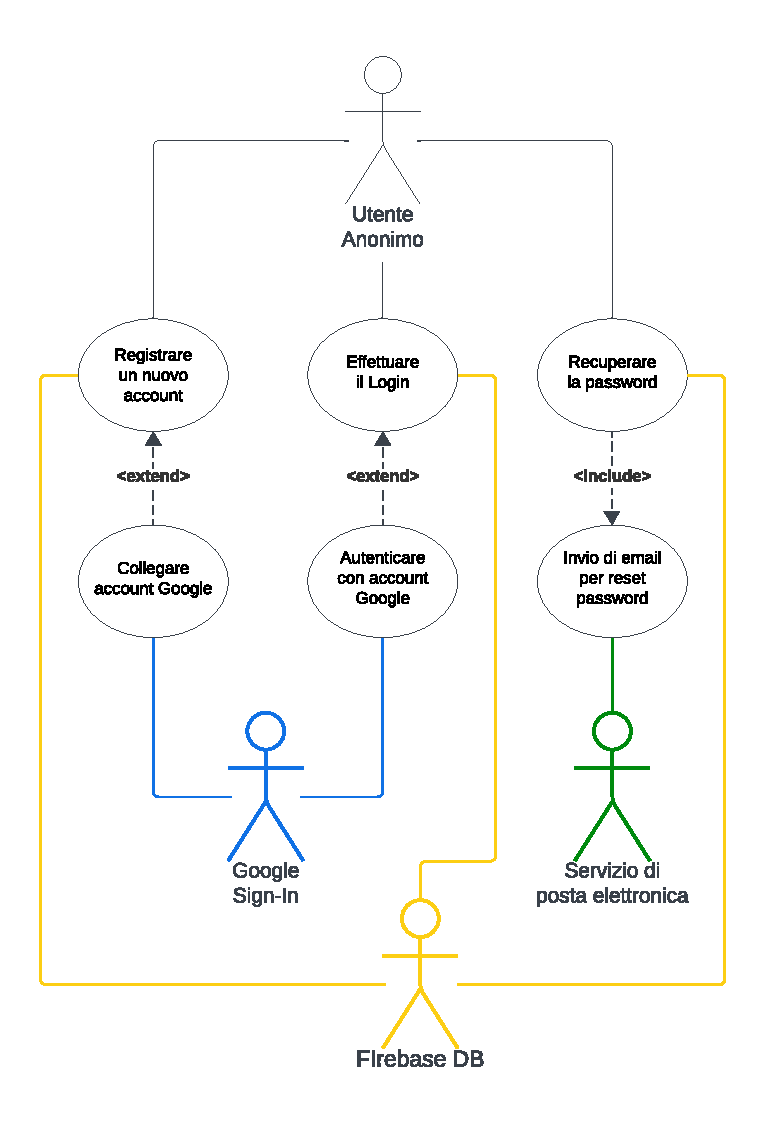
\includegraphics[scale=0.67]{materiale/ucdiagrams/ucaccesso.pdf}
\caption{UCD relativo ai RF inerenti all'accesso alla piattaforma}
\label{access}
\end{figure}

\subsection*{Descrizione Use Case \textit{Registrare un nuovo account}}
\begin{description}
    \item[Titolo:] Registrazione account
    
    \item[Riassunto:] Questo Use Case descrive come l'utente anonimo deve
    effettuare la registrazione sulla piattaforma.

    \item[Descrizione:]
    \begin{enumerate}
        \item[]
        \item L'utente anonimo accede alla pagina dedicata, raggiungibile da quella di login, e sceglie tra la modalità di registrazione con il sistema di credenziali interno oppure per mezzo di un account Google.\texttt{[extension 1]}
        \item La registrazione con sistema di credenziali interno prevede l'inserimento di un username, un'email e una password conforme. \verb|[exception 1]|
        \item La password deve essere confermata reinserendola in un secondo campo.\verb|[exception 2]|
        \item I dati vengono raccolti e il relativo account viene registrato dal servizio di database.\texttt{[exception 3]}
    \end{enumerate}
    
    \item[Exceptions:]
    \begin{itemize}
        \item[]
        \item \texttt{[exception 1]} Se la password non è conforme, la registrazione non può proseguire e l'utente viene avvisato.
        \item \texttt{[exception 2]} Se i campi di inserimento e di conferma della password contengono stringhe che non coincidono, la registrazione non può proseguire e l'utente viene avvisato.
        \item \texttt{[exception 3]} Se l'email inserita dall'utente risulta essere già impiegata in un altro account, la registrazione non può proseguire e l'utente viene avvisato.
    \end{itemize}

    \item[Extensions:]
    \begin{itemize}
        \item[]
        \item \texttt{[extension 1]} L'utente può scegliere di registrarsi alla piattaforma collegando un proprio account Google, secondo quanto indicato dal servizio di registrazione e autenticazione Google.
        In questo caso, oltre a scegliere l'email come previsto dal servizio di Google, l'utente specifica l'username.
    \end{itemize}
\end{description}

\newpage
\subsection*{Descrizione Use Case \textit{Effettuare il login}}
\begin{description}
    \item[Titolo:] Login
    
    \item[Riassunto:] Questo Use Case descrive come l'utente anonimo e registrato deve
    effettuare il login sulla piattaforma.

    \item[Descrizione:]
    \begin{enumerate}
        \item[]
        \item L'utente anonimo accede alla pagina dedicata e sceglie tra l'autenticazione mediante il sistema di credenziali interno oppure per mezzo di un account Google.\texttt{[extension 1]}
        \item L'utente che si autentica con credenziali interne inserisce indirizzo email e password, che saranno verificati grazie al servizio di database.\texttt{[exception 1]}
    \end{enumerate}
    
    \item[Exceptions:]
    \begin{itemize}
        \item[]
        \item \verb|[exception 1]| Se le credenziali fornite non sono valide, il login non può essere eseguito e l'utente viene avvisato.
    \end{itemize}

    \item[Extensions:]
    \begin{itemize}
        \item[]
        \item \texttt{[extension 1]} Qualora l'utente disponga di un account Google collegato alla piattaforma, è possibile effettuare il login
        mediante autenticazione Google e seguendo le indicazioni fornite dal suo servizio.
    \end{itemize}
\end{description}

\subsection*{Descrizione Use Case \textit{Recuperare la password}}
\begin{description}
    \item[Titolo:] Recupero password
    
    \item[Riassunto:] Questo Use Case descrive come l'utente anonimo e
    registrato alla piattaforma, facendo affidamento al sistema di credenziali
    interno, può recuperare il proprio account qualora la password venisse dimenticata.

    \item[Descrizione:]
    \begin{enumerate}
        \item[]
        \item L'utente accede alla pagina di recupero, attraverso quella di login.
        \item La pagina indica all'utente di inserire l'email di recupero, ovvero quella associata all'account. \verb|[exception 1]|
        \item Il sistema richiede al servizio di posta elettronica l'invio di un link di recupero mediane un messaggio email, specificando l'indirizzo fornito dall'utente e il contenuto del messaggio.
        \item Il link guida l'utente dal messaggio alla pagina del sistema dedicata alla creazione di una nuova password.
        \item L'utente inserisce una nuova password conforme e la conferma, inserendola nuovamente. \verb|[exception 2]|
        \item Il servizio di database provvede all'aggiornamento della password.
    \end{enumerate}
    
    \item[Exceptions:]
    \begin{itemize}
        \item[]
        \item \verb|[exception 1]| Se l'email inserita non è associata ad alcun account registrato, il recupero non può proseguire e l'utente viene avvisato.
        \item \verb|[exception 2]| Se la password non è conforme, oppure se i campi di inserimento e conferma della password contengono stringhe che non coincidono, la registrazione non può proseguire e l'utente viene avvisato.
    \end{itemize}
    
    %\item[Extensions:]
\end{description}


\newpage
\subsection{Consultazione dei problemi e profilo}
In Figura \ref{catalogueprobs} sono mostrati gli use cases che illustrano
le funzionalità che interessano l'utente (anonimo, autenticato e amministratore)
nell'ambito della constultazione e manipolazione del catalogo e del contenuto
dei problemi. In particolar modo, sono stati isolate nel diagramma le funzionalità
fruibili nella home page e nella pagina di consultazione
del singolo problema (si vedano \textbf{FE 3}, \textbf{FE 4} e \textbf{FE pagina edit catalogo} nel documento D1).

I requisiti descritti sono: \textbf{RF 5} - Consultazione del catalogo,
\textbf{RF 6} - Consultazione di un problema, \textbf{RF 10} - Metadati aggiuntivi,
\textbf{RF 11.2} - Visualizzare i Progressi, \textbf{RF 14}  Aggiungere un problema,
\textbf{RF 15} - Modificare un problema, \textbf{RF 16} - Eliminare un problema.
Questi ultimi tre, relativi all'utente amministratore, sono riassunti nello use case
\textit{Modificare il catalogo dei problemi}, che include le tre azioni opzionali (da
cui le clausole \texttt{extend} nel diagramma).


\begin{figure}[H]
\centering
\hspace*{-1.5cm}
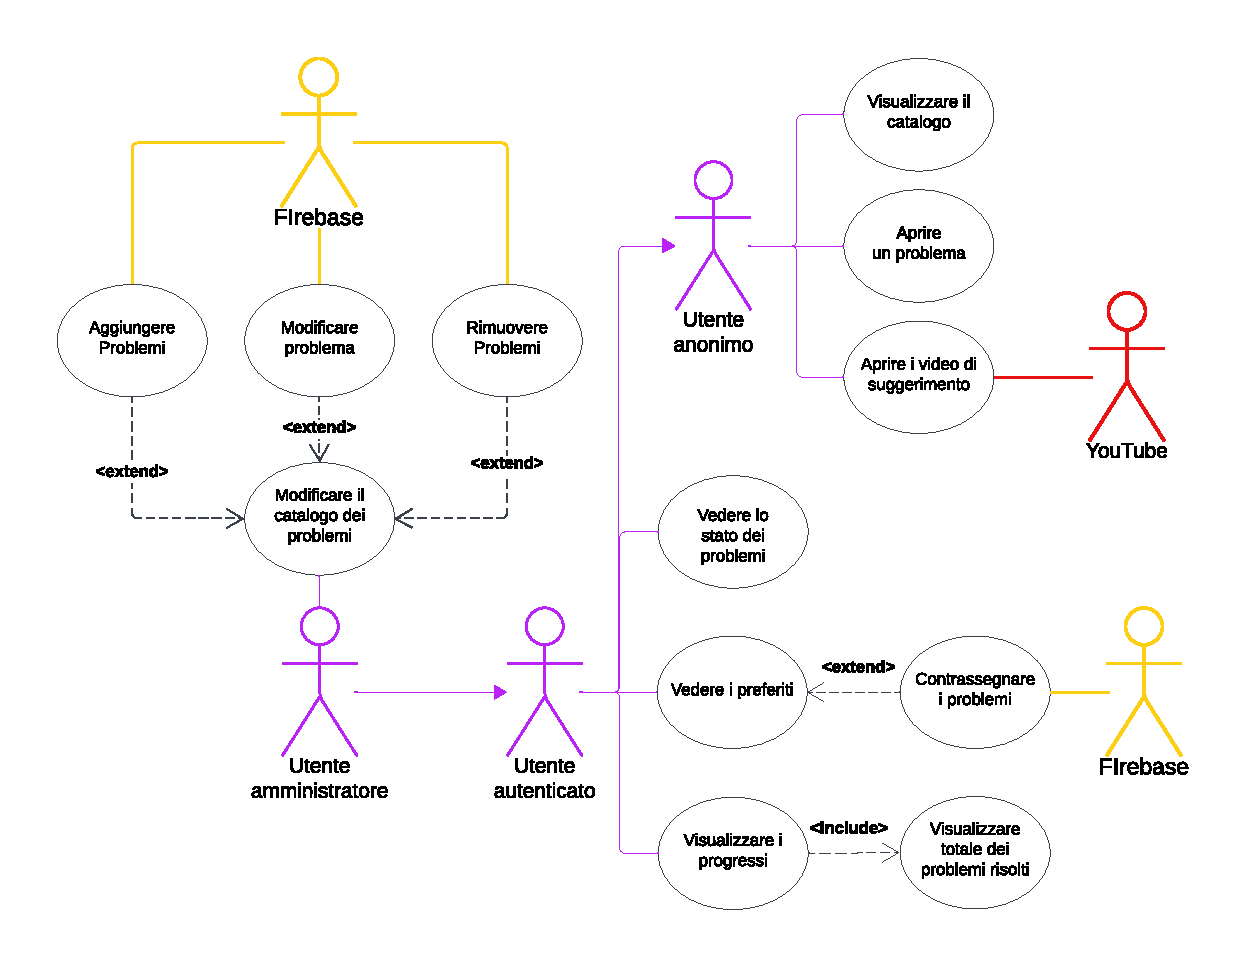
\includegraphics[scale=0.68]{materiale/ucdiagrams/ucproblemi.pdf}
\caption{UCD relativo alla consultazione dei problemi, modifica del catalogo e visualizzazione progressi}
\label{catalogueprobs}
\end{figure}

\newpage
\subsection*{Descrizione Use Case \textit{Aggiungere problemi}}
\begin{description}
    \item[Titolo:] Aggiungere un problema
    
    \item[Riassunto:] Questo Use Case descrive come l'utente amministratore
    deve aggiungere nuovi problemi al catalogo.

    \item[Descrizione:]
    \begin{enumerate}
        \item[]
        \item L'utente amministratore accede alla pagina del catalogo e sceglie di aggiungere un nuovo problema.
        \item L'utente compila i campi necessari alla creazione di un nuovo problema: i dati relativi alla struttura, quali titolo, descrizione e almeno due esempi di input e output atteso; dati descrittivi, ovvero nome, selezione della difficoltà (bassa, intermedia, alta), categoria e link al video-suggerimento.
        \item L'utente inserisce almeno 3 test cases; ogni test case consiste in un dato in input e il rispettivo output corretto.
        \item L'utente conferma la creazione del problema, che viene quindi aggiunto al catalogo; alternativamente, l'utente può scegliere di annullare la creazione del nuovo problema, previo avviso e conferma da parte del sistema.\texttt{[exception 1]}\texttt{[exception 2]}
    \end{enumerate}
    
    \item[Exceptions:]
    \begin{itemize}
        \item[]
        \item \texttt{[exception 1]} Se tra i dati strutturali e descrittivi del problema è presente almeno un campo non compilato, l'aggiunta del problema al catalogo non viene eseguita e l'utente viene avvisato.
        \item \texttt{[exception 2]} Se il numero di test cases forniti è minore di 3, il problema non può essere aggiunto e l'utente viene notificato.
    \end{itemize}
\end{description}

\subsubsection*{Descrizione Use Case \textit{Modificare problemi}}
\begin{description}
    \item[Titolo:] Modificare un problema
    
    \item[Riassunto:] Questo Use Case descrive come l'utente amministratore
    deve modificare i problemi.

    \item[Descrizione:]
    \begin{enumerate}
        \item[]
        \item L'utente amministratore accede alla pagina del catalogo e seleziona un problema da modificare.
        \item L'utente modifica i campi strutturali (titolo, descrizione, esempi di input e output) e descrittivi (nome, difficoltà, categoria e link al video-suggerimento) del problema.
        \item L'utente modifica i test cases, aggiungendone eventualmente più di 3.
        \item L'utente conferma la modifica del problema, che verrà poi aggiornato nel catalogo, oppure conferma di annullare la modifica.\texttt{[exception 1]} \texttt{[exception 2]}
    \end{enumerate}
    
    \item[Exceptions:]
    \begin{itemize}
        \item[]
        \item \texttt{[exception 1]} Se tra i dati strutturali e descrittivi del problema è presente almeno un campo non compilato, la modifica del problema non viene eseguita e l'utente viene avvisato.
        \item \texttt{[exception 2]} Se il numero di test cases forniti è minore di 3, il problema non può essere modificato e l'utente viene notificato.
    \end{itemize}
\end{description}

\newpage
\subsection{Esercitazione e strumenti integrati}
La Figura \ref{esercitaz} raggruppa use cases associati ai requisiti funzionali
che in qualche modo fanno parte del contesto di esercitazione su uno specifico problema. Pertanto,
i requisiti rappresentati qui sono i seguenti: \textbf{RF 7} - Effettuare l'esercitazione,
\textbf{RF 8} - Verifica della correttezza dell'algoritmo, \textbf{RF 11.1} - Registrazione dei
Progressi. Tra gli altri strumenti disponibili insieme all'esercitazione,
vengono anche inclusi in questo diagramma gli use cases associati al
\textbf{RF 9} - Cronometro (si ricorda che il cronometro è indipendente dagli
use cases dell'esercitazione, come appunto rispecchiato nel diagramma).

\begin{figure}[H]
\centering
\hspace*{-1.8cm}
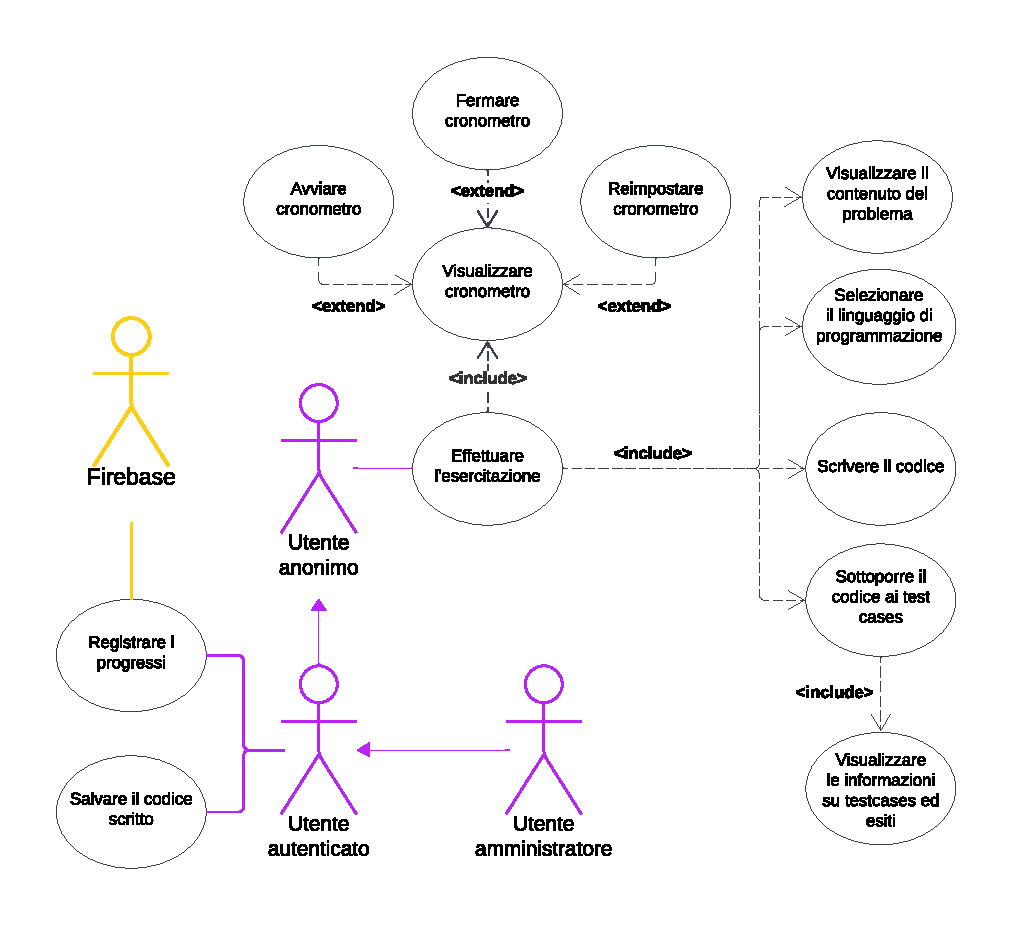
\includegraphics[scale=0.94]{materiale/ucdiagrams/ucesercitazione.pdf}
\caption{UCD con riferimenti ai requisiti relativi all'esercitazione}
\label{esercitaz}
\end{figure}

\newpage
\subsection*{Descrizione dell'esercitazione}
La complessità di alcune operazioni relative all'esercitazione è
catturata dalla Figura \ref{acexercise}.
Dal momento che l'utente può decidere di uscire dall'area di esercitazione
a propria discrezione, si sottolinea che il processo descritto nel diagramma
può essere interrotto in qualsiasi momento—ciò è indicato dalla codizione
\textit{Esci} nel diagramma. La corsia \textit{Firebase} descrive le
attività previste dallo use case \textit{Registrare i progressi}
presente in Figura \ref{esercitaz}.

\begin{figure}[H]
\centering
\hspace*{-1cm}
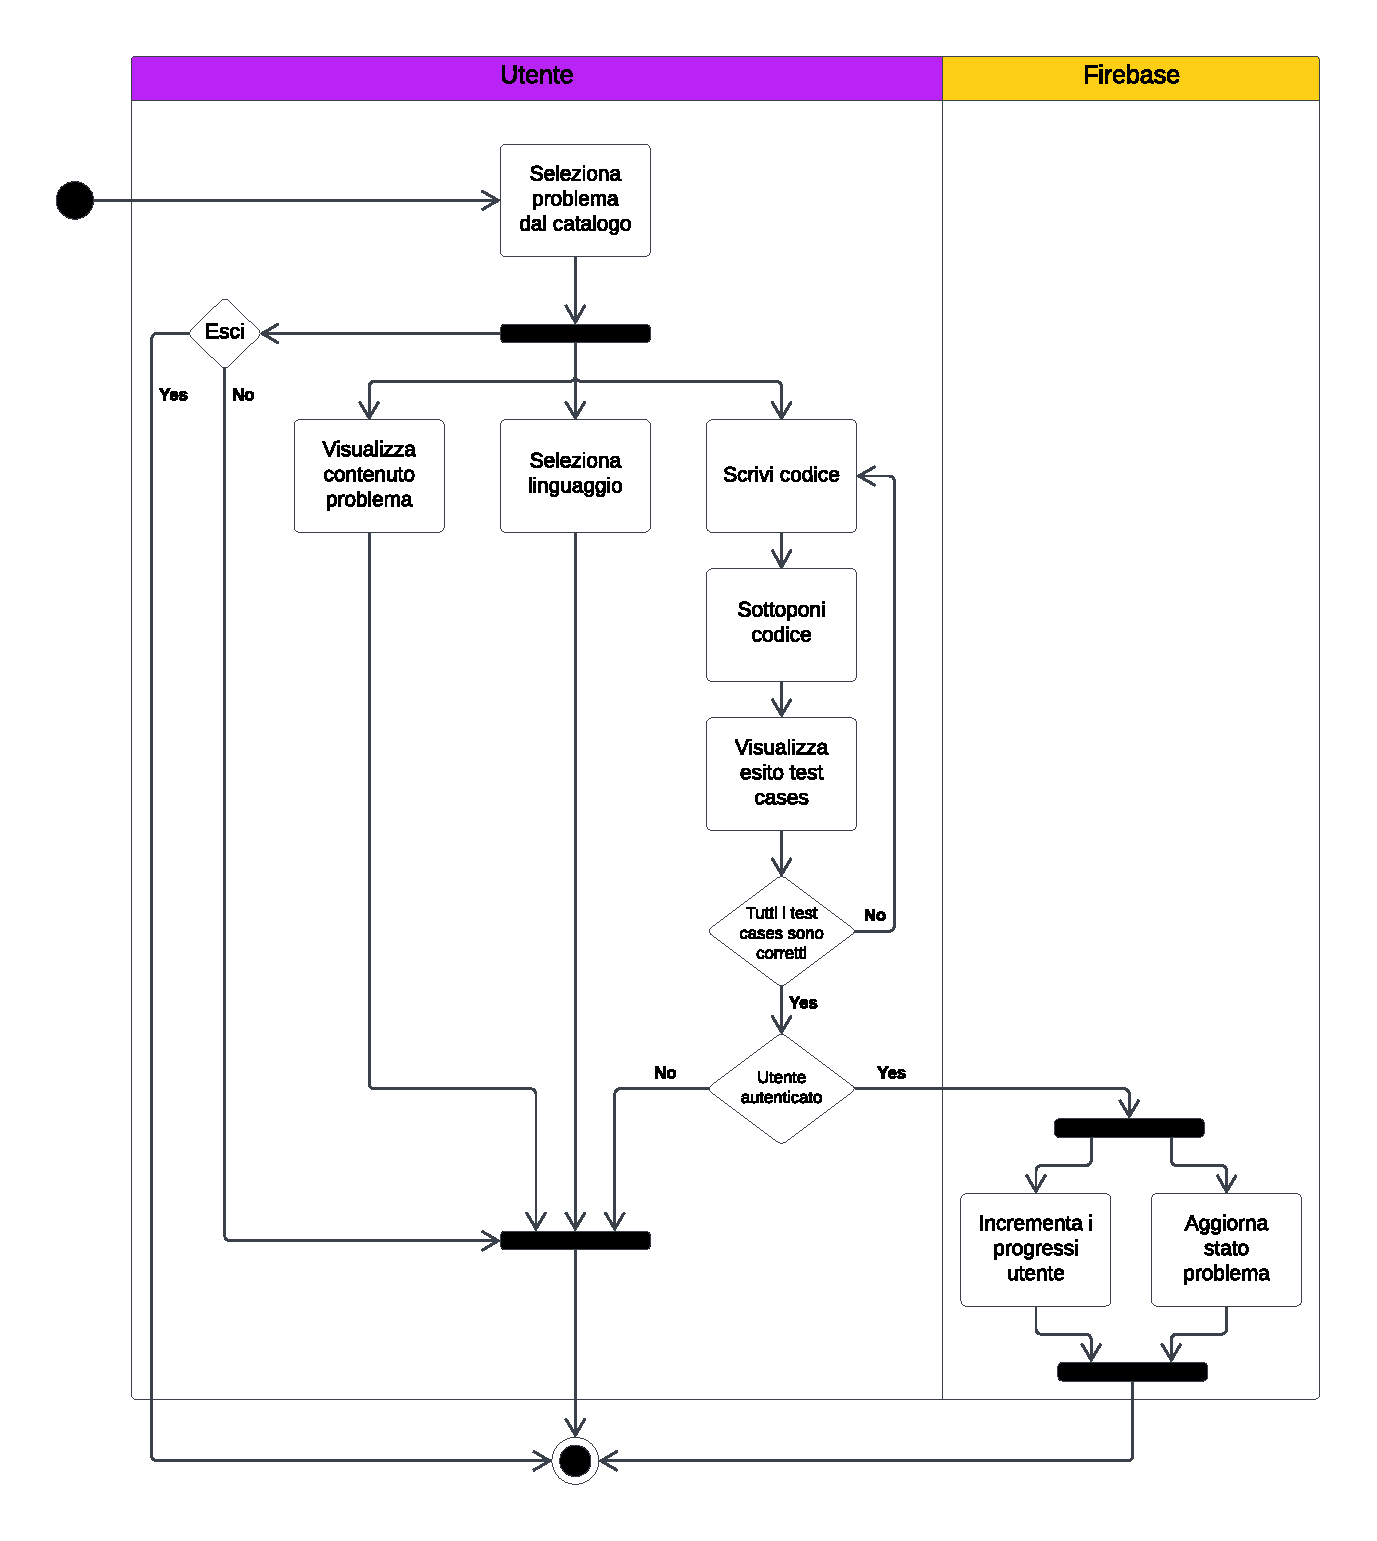
\includegraphics[scale=0.6]{materiale/sldesercitazione.pdf}
\caption{SD, arricchito da elementi di Activity Diagram,
per gli use case \textit{Effetuare l'esercitazione}, gli use case correlati
e \textit{Registrare i progressi}}
\label{acexercise}
\end{figure}


\newpage
\subsection{Gestione dell'account}
In Figura \ref{accountfig} sono riassunti gli use cases che descrivono
le operazioni possibili per gli utenti dotati di account. Come già accennato
nel documento D1, \textit{Aggiornare l'indirizzo email dell'account} e
\textit{Aggiornare la password dell'account} sono possibili solo a utenti
autenticati con sistema di credenziali interno. Questo fatto è appunto
sottolineato dalla presenza dell'attore \textit{Firebase}. Si fa riferimento
ai seguenti requisiti funzionali:
\textbf{RF 12} - Aggiornamento account, \textbf{RF 13} - Logout

\begin{figure}[H]
\centering
%\hspace*{-1.8cm}
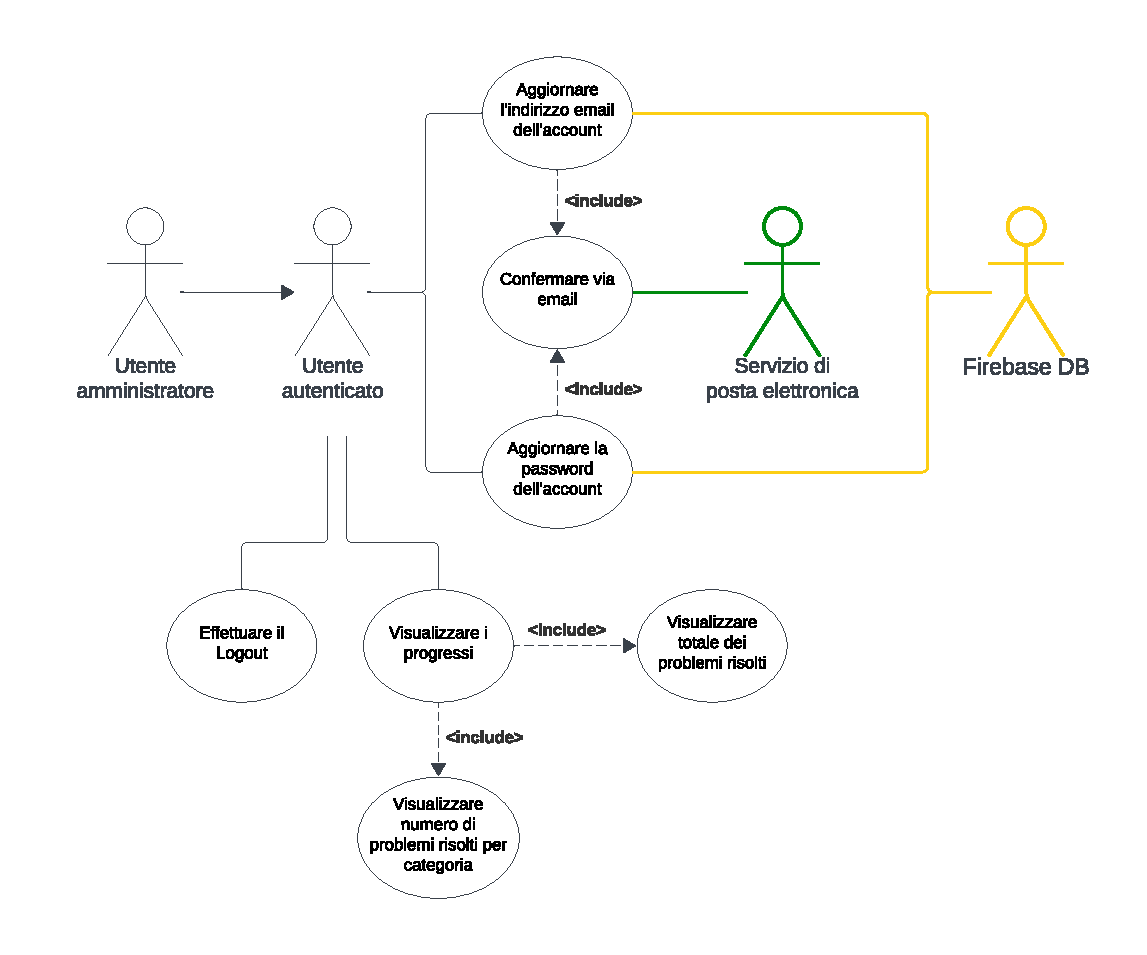
\includegraphics[scale = 0.95]{materiale/ucdiagrams/ucaccount.pdf}
\caption{UCD relativo alle funzionalità dell'account}
\label{accountfig}
\end{figure}



\newpage
\subsection*{\textit{Aggiornare l'indirizzo email dell'account}}
La Figura \ref{slemail} mostra nel dettaglio lo Use Case relativo all'aggiornamento
dell'indirizzo di posta elettronica di un utente registrato con credenziali di sistema
e autenticato, evidenziando i passi della procedura mediante uno Swimlane Diagram.
Le condizioni \textit{annulla operazione} e \textit{conferma operazione}
sottolineano il fatto che l'utente può interrompere la procedura di migrazione
qualora lo ritenga opportuno. In più, viene specificato il comportamento che
il sistema assume nel caso in cui venga inserita un'email già associata ad un
altro account registrato sulla piattaforma.

\begin{figure}[H]
\centering
\hspace*{-1cm}
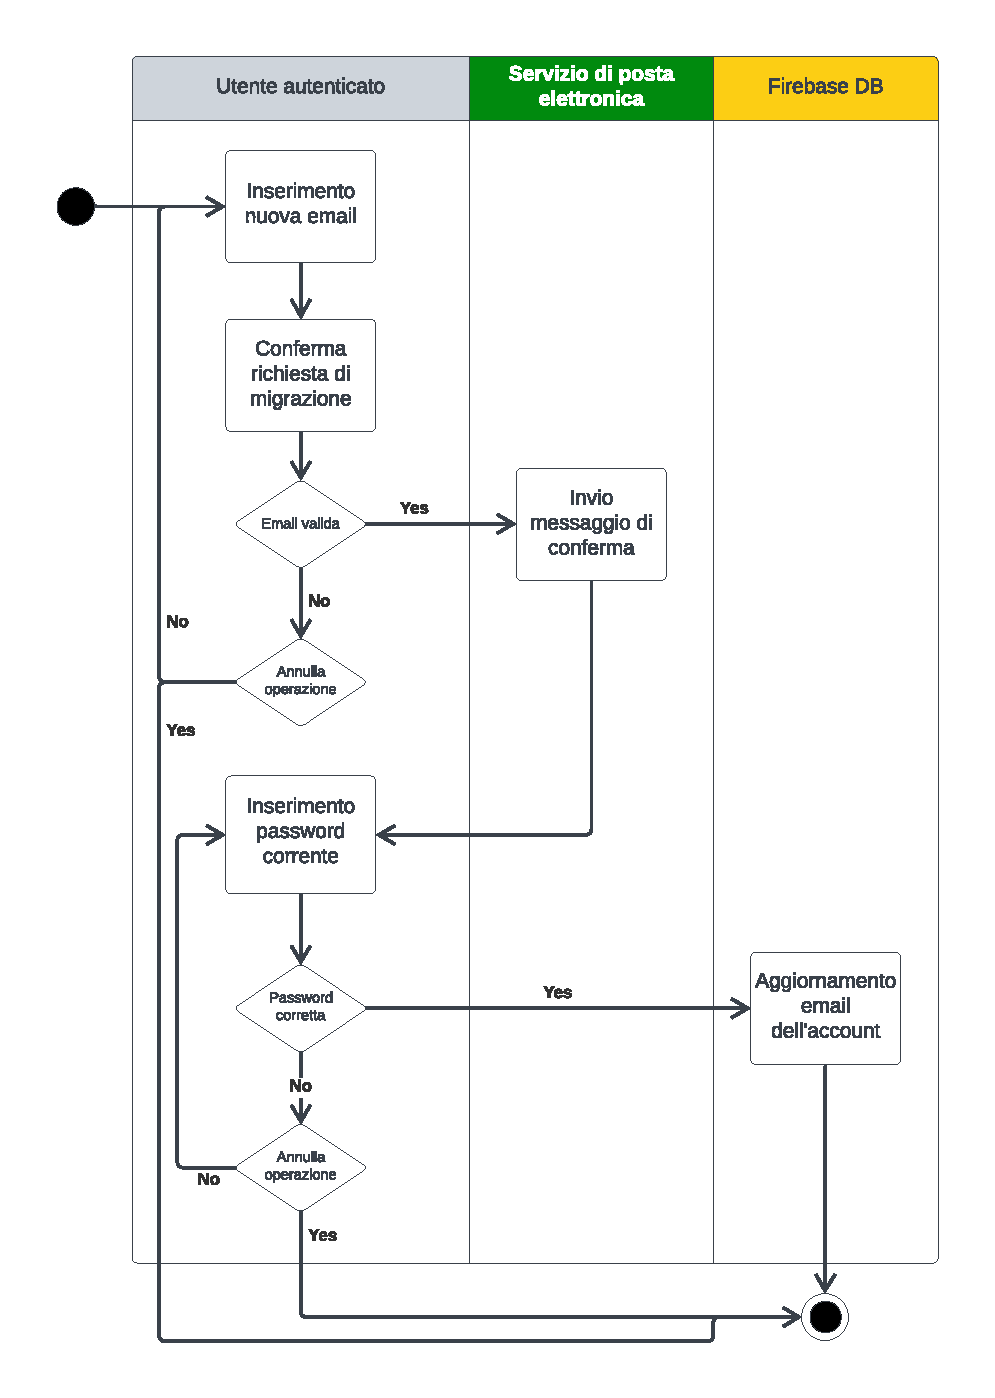
\includegraphics[scale = 0.85]{materiale/ucdiagrams/swimlaneemail.pdf}
\caption{SD dello scenario di aggiornamento dell'indirizzo email}
\label{slemail}
\end{figure}

\subsection*{\textit{Aggiornare la password dell'account}}
La Figura \ref{slpassword} fa riferimento allo Use Case relativo all'aggiornamento
della password dell'account di un utente registrato con credenziali di sistema e autenticato.
Durante il processo di aggiornamento, l'utente ha la facoltà di interrompere
la procedura qualora non intenda più modificare la password. Da qui il
significato delle condizioni \textit{annulla operazione} e \textit{conferma
operazione}.

\begin{figure}[H]
\centering
\hspace*{-0.7cm}
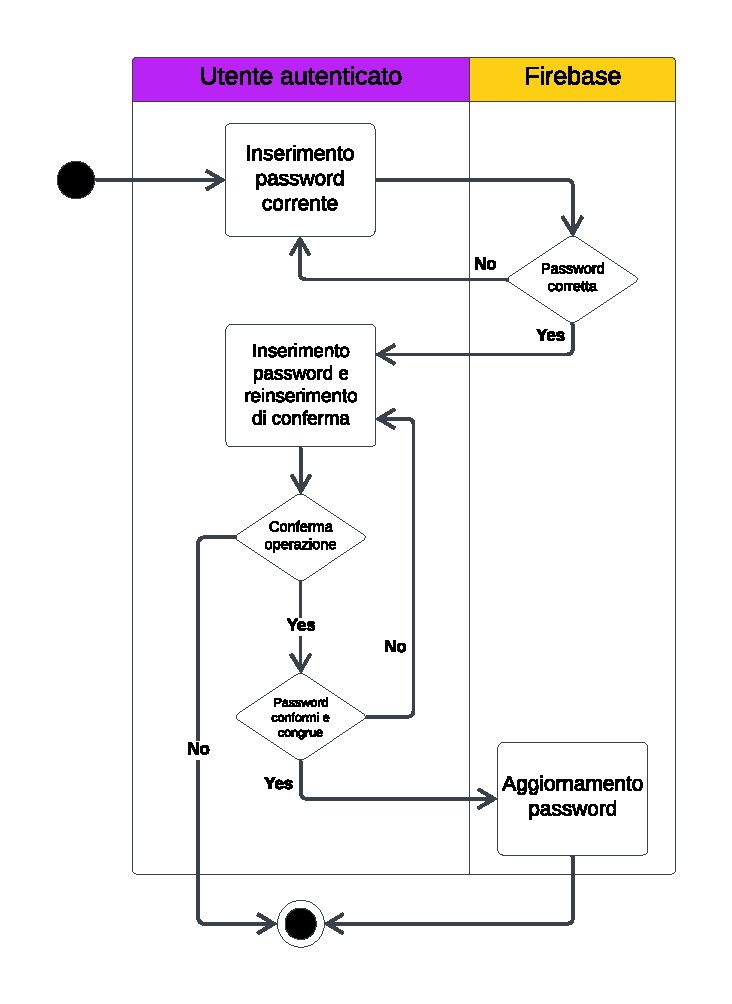
\includegraphics[scale = 0.95]{materiale/ucdiagrams/swimlanepassword.pdf}
\caption{SD dello scenario di aggiornamento della password}
\label{slpassword}
\end{figure}


\newpage
\section{Requisiti non funzionali}
Di seguito sono riportati i requisiti non funzionali (RNF)
del sistema, all'interno di tabelle strutturate. Per ogni requisito vengono
specificate una o più proprietà con una descrizione più esplicita,
oltre ad un indice di misura utile alla valutazione oggettiva
e quantitativa di tali requisiti.

\subsection{Caratteristiche di sistema}

\begin{nonfuncreq}
\textbf{Scalabilità }
\begin{center}
    \footnotesize
    \begin{tabularx}{\textwidth}{|X||X||X|}
        \hline
        \cellcolor{red!70}Proprietà & \cellcolor{red!70}Descrizione & \cellcolor{red!70}Misura\\
        \hline
        Elaborazione con un numero crescente di utenti. & Capacità del sistema di gestire un numero crescente di utenti in simultanea. & Viene garantito l'accesso in simultanea di almeno 300 utenti nel primo anno dal lancio.\\
        \hline
        Memorizzazione dei dati degli utenti & Capacità del sistema di gestire i dati generati da un numero crescente di utenti utilizzatori. & Capacità sufficiente per almeno 400 utenti.\\
        \hline
        Eterogeneità dei linguaggi di programmazione & Capacità di supportare un numero crescente di linguaggi di programmazione, utili alla scrittura degli algoritmi risolutivi. & Al lancio della piattaforma, vengono supportate le versioni maggiormente utilizzate dei linguaggi di programmazione più popolari (C++11). Il sistema può gestire algoritmi scritti in almeno 5 linguaggi differenti.\\
        \hline
    \end{tabularx}
\end{center}
\end{nonfuncreq}

\begin{nonfuncreq}
    \textbf{Compatibilità }
    \begin{center}
        \footnotesize
        \begin{tabularx}{\textwidth}{|X||X||X|}
            \hline
            \cellcolor{red!70}Proprietà & \cellcolor{red!70}Descrizione & \cellcolor{red!70}Misura\\
            \hline
            Compatibilità client & La piattaforma del servizio deve essere compatibile con e accessibile attraverso le versioni più recenti dei principali browser in commercio. &
            \begin{itemize}
                \item Chrome

                117.0.5938.150
                \item Firefox

                18.0.1
                \item Edge:

                17.0.2045.60
            \end{itemize}La compatibilità deve valere anche per le rispettive versioni superiori.\\
            \hline
        \end{tabularx}
    \end{center}
\end{nonfuncreq}

\begin{nonfuncreq}
    \textbf{Usabilità }
    \begin{center}
        \footnotesize
        \begin{tabularx}{\textwidth}{|X||X||X|}
            \hline
            \cellcolor{red!70}Proprietà & \cellcolor{red!70}Descrizione & \cellcolor{red!70}Misura\\
            \hline
            Usabilità & Intuitività e facilità nell'apprendimento, accesso e impiego delle funzionalità fornite dal servizio. & Il nuovo utente deve poter conoscere e utilizzare il 90\% delle funzionalità (disponibili al proprio livello di accesso) in meno di 30 minuti.\\
            \hline
        \end{tabularx}
    \end{center}
\end{nonfuncreq}

\begin{nonfuncreq}
    \textbf{Aspetto }
    \begin{center}
        \footnotesize
        \begin{tabularx}{\textwidth}{|X||X||X|}
            \hline
            \cellcolor{red!70}Proprietà & \cellcolor{red!70}Descrizione & \cellcolor{red!70}Misura\\
            \hline
            Colore & Gamma cromatica dell'interfaccia e distribuzione del colore. La scelta ricade su colori, tinte (aggiunta di bianco) e sfumature (aggiunta di nero) che mirano a limitare l'affaticamento della vista. & Colori caldi; colori freddi presenti in sfumature scure; colori freddi accesi presenti al più in aree ristrette (pulsanti e icone).\\
            \hline
            Contrasto & Accostamento dei colori all'interno dell'interfaccia utente. Mira alla leggibilità e alla limitazione dell'affaticamento della vista. & Regola dei complementari; cerchio di Itten.\\
            \hline
        \end{tabularx}
    \end{center}
\end{nonfuncreq}

\begin{nonfuncreq}
    \textbf{Lingua }
    \begin{center}
        \footnotesize
        \begin{tabularx}{\textwidth}{|X||X||X|}
            \hline
            \cellcolor{red!70}Proprietà & \cellcolor{red!70}Descrizione & \cellcolor{red!70}Misura\\
            \hline
            Lingua di sistema           & Lingua presente nell'interfaccia e nelle risorse fornite dal servizio. & L'interfaccia generale della piattaforma contiene testo in italiano (100\%); i testi dei problemi sono scritti in italiano (100\%); le risorse multimediali (video-suggerimento) devono essere in italiano oppure in inglese.\\
            \hline
        \end{tabularx}
    \end{center}
\end{nonfuncreq}

\begin{nonfuncreq}
    \textbf{Prestazioni }
    \begin{center}
        \footnotesize
        \begin{tabularx}{\textwidth}{|X||X||X|}
            \hline
            \cellcolor{red!70}Proprietà & \cellcolor{red!70}Descrizione & \cellcolor{red!70}Misura\\
            \hline
            Caricamento all'accesso & Tempo massimo richiesto per caricare le pagine rilevanti dopo la ricerca in browser. & Il caricamento delle pagine di login e home (per quest'ultima si considera l'intervallo di tempo che comincia dopo la richiesta di autenticazione) non deve eccedere i 2 secondi.\\
            \hline
            Transizioni & Tempo massimo richiesto per effettuare una transizione da una pagina all'altra.  & Una transizione non deve richiedere più di 2 secondi.\\
            \hline
        \end{tabularx}
    \end{center}
\end{nonfuncreq}

\subsection{Affidabilità}

\begin{nonfuncreq}
    \textbf{Downtime }
    \begin{center}
        \footnotesize
        \begin{tabularx}{\textwidth}{|X||X||X|}
            \hline
            \cellcolor{red!70}Proprietà & \cellcolor{red!70}Descrizione & \cellcolor{red!70}Misura\\
            \hline
            Downtime & Tempo medio massimo in cui il servizio non è raggiungibile; principalmente per motivi di manutenzione e aggiornamento. & 2,7\% (240 ore) nel primo anno 0,85\% (72 ore) dopo il primo anno dal lancio.\\
            \hline
        \end{tabularx}
    \end{center}
\end{nonfuncreq}

\begin{nonfuncreq}
    \textbf{Disponibilità }
    \begin{center}
        \footnotesize
        \begin{tabularx}{\textwidth}{|X||X||X|}
            \hline
            \cellcolor{red!70}Proprietà & \cellcolor{red!70}Descrizione & \cellcolor{red!70}Misura\\
            \hline
            Disponibilità & Probabilità che il sito non si guasti entro un intervallo di tempo trascorso dopo l'entrata in servizio. & Probabilità di resistere ai guasti al 98\% entro le prime 8.000 ore.\\
            \hline
        \end{tabularx}
    \end{center}
\end{nonfuncreq}

\subsection{Privacy e sicurezza}

\begin{nonfuncreq}
    \textbf{Privacy e trattamento dei dati }
    \begin{center}
        \footnotesize
        \begin{tabularx}{\textwidth}{|X||X||X|}
            \hline
            \cellcolor{red!70}Proprietà & \cellcolor{red!70}Descrizione & \cellcolor{red!70}Misura\\
            \hline
            Normativa & Conformità con le vigenti norme relative al trattamento e alla protezione dei dati (GDPR). In particolare, i dati personali dell'utente registrato (nome, email e password) non devono essere divulgati in alcun modo e, qualora lo ritenga opportuno, l'utente ha il diritto di richiedere l'eliminazione delle proprie informazioni dal servizio al fine di interrompere il trattamento. & Conformità del servizio e funzionalità a supporto dell'utente (eliminazione account).\\
            \hline
        \end{tabularx}
    \end{center}
\end{nonfuncreq}

\begin{nonfuncreq}
    \textbf{Connessione sicura }
    \begin{center}
        \footnotesize
        \begin{tabularx}{\textwidth}{|X||X||X|}
            \hline
            \cellcolor{red!70}Proprietà & \cellcolor{red!70}Descrizione & \cellcolor{red!70}Misura\\
            \hline
            Connessione sicura & Impiego di protocolli di comunicazione che garantiscono la confidenzialità e riservatezza delle informazioni scambiate tra client e server. & Utilizzo del protocollo \texttt{https}.\\
            \hline
        \end{tabularx}
    \end{center}
\end{nonfuncreq}

\begin{nonfuncreq}
    \textbf{Password strength }
    \begin{center}
        \footnotesize
        \begin{tabularx}{\textwidth}{|X||X||X|}
            \hline
            \cellcolor{red!70}Proprietà & \cellcolor{red!70}Descrizione & \cellcolor{red!70}Misura\\
            \hline
            Password sicura & Quantità e varietà di caratteri necessari per comporre una password forte. & Una password conforme possiede da 8 a 64 caratteri, tra i quali sono presenti almeno: una lettera maiuscola, una minuscola, una cifra decimale e un carattere speciale tra ! ? \# \$ \% \& @ * + - / $\backslash$ = \_ . , ; : ( ) [ ] \{ \}.\\
            \hline
        \end{tabularx}
    \end{center}
\end{nonfuncreq}





\newpage
\section{Analisi del contesto}
% riguarda il backend e i componenti esterni al sistema: tutto il codice che utilizzate ma che non avete scritto voi
% flusso di informazioni tra il nostro sistema e quelli esterni
In questa sezione viene descritto il contesto di funzionamento del sistema
\textit{SleepCode} e come esso interagisce con gli attori esterni. Si
ricorre ad una descrizione testuale riassunta in una rappresentazione
grafica mediante un Diagramma di Contesto (Figura \ref{contextdiagram}),
nel quale sono specificati, ad alto livello, i flussi di informazioni
essenziali al funzionamento del sistema.

\subsection{Utenti e sistemi esterni} % chi interagisce, chi usa e chi supporta (sia software che umano)
Sono elencati di seguito gli attori esterni che compongono il contesto
del sistema in sviluppo. Essi fanno riferimento ad alcuni dei requisiti
funzionali definiti nel documento D1.

\subsubsection{Utente}
L'utente rappresenta l'attore che usufruisce delle funzionalità del servizio
—viene descritto nei requisiti dal \textbf{RF 1} al \textbf{RF 9} per quanto
concerne il livello anonimo e quelli superiori; dal \textbf{RF 10} al
\textbf{RF 13} in relazione ai livelli autenticato e amministratore; \textbf{RF 14},
\textbf{RF 15} e \textbf{RF 16} per quanto riguarda il livello amministratore.

\subsubsection{Firebase}
Il servizio di database impiegato per gestire le credenziali e il profilo
degli utenti registrati alla piattaforma—i requisiti coinvolti sono: \textbf{RF 1},
\textbf{RF 2}, \textbf{RF 3}, \textbf{RF 4}, \textbf{RF 9}, \textbf{RF 10}—e per gestire il
catalogo dei problemi—\textbf{RF 14}, \textbf{RF 15}, \textbf{RF 16}.

\subsubsection{Google Sign-In}
Il servizio di autenticazione alternativo al sistema di credenziali interno
—\textbf{RF 3}.

\subsubsection{YouTube}
Il servizio di contenuti multimediali che fornisce i video che integrano
i problemi del catalogo, mettendo a disposizione dell'utente un suggerimento per lo
svolgimento dell'esercizio—\textbf{RF 5.1}.
%\textbf{RF 7.5}??

\subsubsection{Servizio di posta elettronica}
Sistema di notifica sul quale il progetto si poggia per creare un
meccanismo di recupero dell'account—\textbf{RF 4}.

\newpage
\subsection{Diagramma di contesto} % frecce = dati che si scambiano. Utente --atuenticaz--> sistema (è l'utente che fornisce i dati al sistema; la freccia indica il verso del flusso)
La Figura \ref{contextdiagram} mostra il diagramma di contesto per il
servizio \textit{SleepCode}. Seguono alcune descrizioni più dettagliate,
che chiariscono il significato delle informazioni scambiate tra il sistema
e gli attori esterni ad esso, facendo anche riferimento ai requisiti
funzionali che vengono soddisfatti grazie a tali interazioni.

\begin{figure}[H]
\centering
\hspace*{-2.4cm}
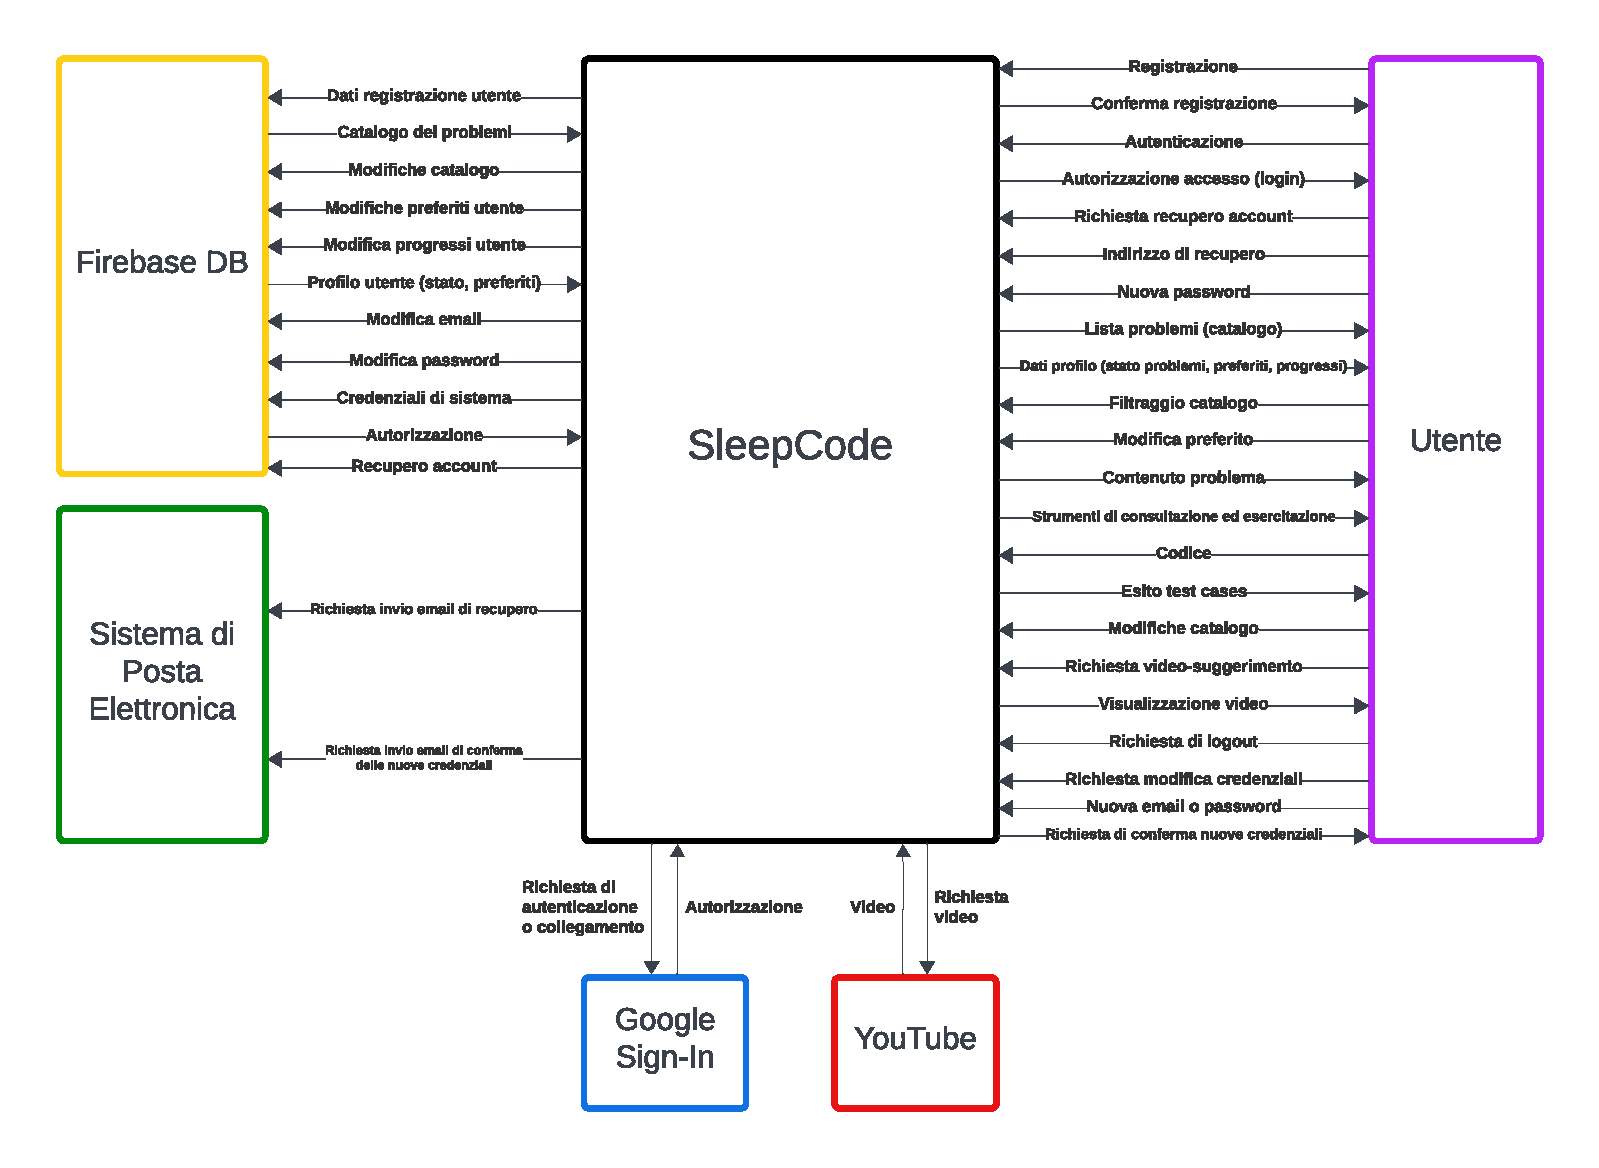
\includegraphics[scale=0.65]{materiale/contextdiagram.pdf}
\caption{Context Diagram della piattaforma \textit{SleepCode}}
\label{contextdiagram}
\end{figure}

\subsubsection*{Utente}
L'utente può richiedere di effettuare la registrazione alla piattaforma
(\textbf{RF 1}), scegliendo di inviare i dati necessari per creare un
account di sistema o di collegare il proprio account Google. Il sistema
provvede a inviare la conferma dell'operazione di registrazione.

L'utente registrato può inviare i dati necessari al login (\textbf{RF 2}) sulla piattaforma,
inserendo quindi le credenziali di sistema oppure richiedendo l'autenticazione
con Google. Il sistema risponde con l'autorizzazione all'accesso.

In caso di richiesta di recupero dell'account (\textbf{RF 3}) da parte di un utente
registrato, il sistema riceve l'indirizzo email di recupero. Dall'email
l'utente può collegarsi alla pagina di recupero, nella quale inserire la
nuova password dell'account.

L'utente riceve il catalogo e i dati in esso contenuti (\textbf{RF 4}, \textbf{RF 5},
\textbf{RF 8}). L'utente propaga al proprio account le modifiche
apportate ai preferiti (\textbf{RF 8}) e al catalogo stesso (\textbf{RF 12}, \textbf{RF 13}, \textbf{RF 14}), riceve le informazioni sui progressi personali (\textbf{RF 9})
e può inviare una richiesta di logout (\textbf{RF 11}). Ovviamente
i dati che realizzano il profilo dell'utente, quali stato dei problemi,
preferiti e progressi, sono visibili all'utente.

Durante un'esercitazione, l'utente può inviare il codice scritto e ricevere dati
relativi all'esito dell'esecuzione di tale codice; può essere inoltre richiesta la
visualizzazione del video-suggerimento (\textbf{RF 6}, \textbf{RF 7}).

Per apportare modifiche ai dati del proprio account (\textbf{RF 10}), l'utente
deve poter inviare le richieste specifiche, come quelle di modifica della password
o migrazione dell'indirizzo email, e fornire le nuove credenziali. Il
sistema richiede la conferma di tali operazioni mediante l'invio, da parte
dell'utente, delle opportune credenziali.

\subsubsection*{Firebase}
Firebase provvede alla memorizzazione del catalogo (con relativi problemi) e dei
dati associati agli utenti registrati ed eventualmente autenticati (credenziali
interne, preferiti, progressi) e alla ricezione di modifiche apportate a questi oggetti.

\subsubsection*{Google Sign-In}
Google Sign-In fornisce l'autorizzazione al collegamento e all'accesso
mediante account Google, richiesti da utenti in sede di registrazione o
login.

\subsubsection*{YouTube}
I video che l'utente intende visualizzare vengono richiesti a YouTube da
parte del sistema, per poi visualizzarli.

\subsubsection*{Servizio di posta elettronica}
La piattaforma fornisce al sistema di posta elettronica i dati necessari
per notificare e guidare l'utente che intende effettuare l'operazione di
recupero dell'account.



\newpage
\section{Analisi dei componenti}
% diagramma componenti -> si intende componenti INTERNI AL SISTEMA:

% vantaggi componenti: se cambia uno degli attori (in particolare software)
% basta cambiare il rispettivo compnente con il quale si interfaccia

% il sistema non sarà un programma monolitico che si occupa di tutto con un unico codice
% provo a dividere il mio sistema in componenti e ragiono su come le informazioni vengono passate tra i componenti

Nella sezione seguente viene descritta l'architettura interna del sistema
rilevandone i componenti, definiti nei loro compiti sulla base dei requisiti
analizzati nelle sezioni e nei documenti precedenti. L'architettura viene
qui mostrata attraverso un Diagramma dei Componenti (Figura \ref{compdiagram}), che evidenzia
l'interconnessione tra i componenti interni, le interfacce presenti tra di
essi e quelle esposte agli attori esterni. Segue una descrizione testuale
e più dettagliata di ogni componente.


\subsection{Definizione dei componenti}
In questa sezione sono descritti i componenti e le interfacce presenti
all'interno del Diagramma dei Componenti.

\iffalse
\subsubsection{Pagina di Autenticazione}
\begin{description}
    \item[Descrizione:] questo componente ha il compito
    principale di interagire con l'utente al fine di guidarlo
    nelle procedure di accesso alla piattaforma.
    La Pagina di Autenticazione si occupa della raccolta dei dati
    utili ad effettuare il login e la registrazione
    di un nuovo account. Essa offre inoltre la possibilità di
    richiedere il recupero dell'account.
    \item[Interfacce richieste:]
    \begin{itemize}
        \item[]
        \item \underline{Credenziali:} la pagina di accesso
        richiede l'inserimento delle credenziali necessarie
        per il login (una tupla email-password) e per la
        registrazione (nome utente, email, password).

        \item \underline{Richiesta registrazione:} con tale
        interfaccia esposta all'utente, il componente è in grado
        di distinguere dal login l'operazione di registrazione,
        richiedendo, tramite l'interfaccia Credenziali, i dati
        opportuni.

        \item \underline{Richiesta Google:} con questa interfaccia,
        la Pagina di Autenticazione può riconoscere che l'utente
        intende registrarsi o autenticarsi mediante un account
        Google.

        \item \underline{Autorizzazione:} l'autorizzazione, da
        parte dell'apposito Sistema di Autenticazione, consente
        alla Pagina di Accesso di stabilire se il login o la
        registrazione sono andate a buon fine. In questo modo, si
        conferma all'utente l'accesso alla piattaforma, oppure lo
        si avvisa di eventuali errori.

        \item \underline{Richiesta recupero account:} dalla Pagina
        di Autenticazione, l'utente fornisce una richiesta di
        recupero dell'account qualora la password dovesse essere
        dimenticata. Con questa interfaccia, il componente provvede
        all'avvio della procedura di recupero.
    \end{itemize}
    \item[Interfacce fornite:]
    \begin{itemize}
        \item[]
        \item \underline{Login:} la pagina risponde ad una registrazione
        o autenticazione andata a buon fine portando a termine un'operazione
        di login. Questa interfaccia consente al sistema di distinguere
        la transizione dello stato di un utente da anonimo ad autenticato.

        \item \underline{Credenziali di accesso:} le credenziali per il login,
        raccolte precedentemente, vengono inoltrate a componenti preposti alla
        loro convalida.

        \item \underline{Credenziali di registrazione:} le credenziali necessarie
        alla registrazione, raccolte precedentemente, vengono inoltrate 

        \item \underline{Richiesta Google:} questa interfaccia permette alla
        pagina di accesso di comunicare il fatto che l'utente intende registrarsi
        o autenticarsi con un account Google.

        \item \underline{Richiesta recupero account:} il componente inoltra
        al componente Pagina di Recupero la richiesta di recupero account, in modo
        tale da effettuare separatamente questa operazione.
    \end{itemize}
\end{description}
\fi


\begin{center}
    \rule{5cm}{1pt}
\end{center}


\subsubsection{Home Page}
\begin{description}
    \item[Descrizione:] il componente si occupa di guidare l'utente nella
    navigazione, esponendo dunque sul front-end le funzionalità relative
    al reindirizzamento ad altre pagine: Pagina di Autenticazione, Catalogo, pagina
    di eserictazione e consultazione dei problemi. Se l'utente è autenticato,
    questo componente ha il compito di mostrare i progressi dell'utente.
    \item[Interfacce richieste:]
    \begin{itemize}
        \item[]
        \item \underline{Richiesta pagina di autenticazione:}
        \item \underline{Richiesta catalogo:}
        \item \underline{Richiesta}
    \end{itemize}
\end{description}

\begin{center}
    \rule{5cm}{1pt}
\end{center}

\subsubsection{Pagina di Autenticazione}
\begin{description}
    \item[Descrizione:]

    \item[Interfacce richieste:]
    \begin{itemize}
        \item[]

        \item \underline{Credenziali:}
        \item \underline{Richiesta Google:}
    \end{itemize}

    \item[Interfacce fornite:]
    \begin{itemize}
        \item[]

        \item \underline{Login:}
        \item \underline{Registrazione:}
        \item \underline{Conferma login:}
    \end{itemize}
\end{description}

\begin{center}
    \rule{5cm}{1pt}
\end{center}

\subsubsection{Gestore account}
\begin{description}
    \item[Descrizione:]

    \item[Interfacce richieste:]
    \begin{itemize}
        \item[]

        \item
    \end{itemize}

    \item[Interfacce fornite:]
    \begin{itemize}
        \item[]

        \item
    \end{itemize}
\end{description}

\begin{center}
    \rule{5cm}{1pt}
\end{center}

\subsubsection{Catalogo}
\begin{description}
    \item[Descrizione:] questo componente consente ad un qualsiasi utente
    (anonimo, autenticato e amministratore) di consultare la lista di problemi
    disponibili sulla piattaforma, oltre a permettere di selezionare un singolo
    problema per aprirlo e iniziare a risolverlo, passando quindi alla Pagina di
    Esercitazione (Sezione \ref{exepag}).
    Il Catalogo facilita la navigazione visualizzando i dati descrittivi di ogni
    problema (nome, categoria, difficoltà), permettendo anche di eseguire ricerche
    filtrate per nome o altri campi; consente di visualizzare i suggerimenti senza
    la necessità di aprire il problema; mostra lo stato di ogni problema e i
    preferiti alla vista dell'utente autenticato (e amministratore); fornisce gli
    strumenti utili agli utenti amministratori per aggiungere, modificare ed
    eliminare i problemi del catalogo.

    \item[Interfacce richieste:]
    \begin{itemize}
        \item[]

        \item \underline{Lista dei problemi:} il Catalogo ha il compito di
        mostrare i problemi memorizzati grazie al servizio di database impiegato.
        Per questo motivo, questa interfaccia consente al catalogo di recuperare
        dal database i problemi disponibili.

        \item \underline{Filtro:} il Catalogo rileva i filtri di ricerca selezionati
        dall'utente, cosicché i problemi che corrispondono ai criteri di ricerca possano
        essere visualizzati. I filtri includono la ricerca per nome, per difficoltà e categoria.

        \item \underline{Richiesta suggerimento:} questa interfaccia permette all'utente
        di visualizzare il video-suggerimento associato al problema in questione.

        \item \underline{Video:} il Catalogo interagisce con YouTube per ottenere il
        video-suggerimento da visualizzare su richiesta dell'utente.

        \item \underline{Conferma login:} il Catalogo richiede l'esito dell'operazione di
        login in modo da mostrare i preferiti e lo stato dei problemi associati
        all'utente autenticato.

        \item \underline{Preferiti:} il Catalogo riceve i preferiti dell'utente autenticato,
        in modo da visualizzarli nella lista dei problemi.
        
        \item \underline{Problemi risolti:} il Catalogo riceve i problemi risolti dall'utente,
        cosicché lo stato dei problemi sia visibile nella lista.

        \item \underline{Modifica preferiti:} gli utenti autenticati possono interagire
        con il Catalogo al fine di contrassegnare come preferiti i problemi visualizzati.
        Mediante questa interfaccia è altresì possibile rimuovere un problema dai preferiti.

        \item \underline{Modifica problema:} il Catalogo accetta eventuali modifiche
        che vengono richieste da utenti amministratori. Da questa interfaccia, il
        Catalogo consente agli amministratori di aggiungere, modificare o eliminare
        i problemi del catalogo.
    \end{itemize}

    \item[Interfacce fornite:]
    \begin{itemize}
        \item[]
        
        \item \underline{Lista:} il Catalogo visualizza la lista dei problemi e i
        dati descrittivi affini di ogni problema.

        \item \underline{Visualizzazione suggerimento:} il Catalogo visualizza il
        video suggerimento relativo ad uno specifico problema e richiesto precedentemente
        dall'utente.

        \item \underline{Richiesta problema:} il Catalogo rileva la selezione di
        un problema consentendo all'utente di accedere alla pagina dedicata alla
        consultazione ed esercitazione (Pagina Esercitazione, Sezione \ref{exepag}).
        
        \item \underline{Stato:} lo stato dei problemi risolti è visibile all'utente
        autenticato. Il Catalogo segnala eventuali problemi risolti
        mediante un apposito simbolo in un campo \textit{stato}.

        \item \underline{Preferiti:} i preferiti vengono visualizzati qualora
        l'utente che naviga il Catalogo sia già autenticato. Il Catalogo consente
        di riconoscere i preferiti visualizzando un apposito simbolo in un campo
        \textit{preferiti}.

        \item \underline{Modifiche preferiti:} il Catalogo comunica al database le
        modifiche approtate ai preferiti di un particolare utente.

        \item \underline{Modifiche problemi:} il Catalogo comunica al database eventuali
        modifiche apportate alla lista dei problemi.
    \end{itemize}
\end{description}

%\subsubsection{Video Player?}
%\begin{description}
%    \item[Descrizione:] questo componente si occupa di interagire con l'attore esterno
%    YouTube, inviando le richieste dei video di suggerimento, ricevendo tali video e
%    permettendo la loro visualizzazione sulla piattaforma.
%
%    \item[Interfacce richieste:]
%    \begin{itemize}
%        \item[]
%
%        \item \underline{Richiesta suggerimento:} questa interfaccia permette ad altri
%        componenti interni (Pagina Esercitazione e Catalogo) di inviare le richieste di
%        visualizzazione dei suggerimenti.
%
%        \item \underline{Video:} questa interfaccia rappresenta il punto di ricezione
%        del video di YouTube, che poi verrà visualizzato all'interno della piattaforma.
%    \end{itemize}
%
%    \item[Interfacce fornite:]
%    \begin{itemize}
%        \item[]
%
%        \item \underline{Richiesta video:}
%        \item \underline{Visualizzazione video:}
%    \end{itemize}
%\end{description}

\begin{center}
    \rule{5cm}{1pt}
\end{center}

\subsubsection{Pagina di Esercitazione}\label{exepag}
\begin{description}
    \item[Descrizione:] il componente consente di consultare il contenuto del problema
    precedentemente selezionato nel catalogo. Inoltre, la Pagina di Esercitazione mette
    a disposizione gli strumenti utili alla risoluzione dell'esercizio, provvede alla
    gestione della sottomissione del codice e avvisa l'utente circa la correttezza dell'algoritmo.
    Qualora il codice sia corretto, questo componente si occupa di aggiornare i progressi
    dell'utente (autenticato) che ha risolto il problema, insieme allo stato di quest'ultimo
    in relazione all'utente in esame.

    \item[Interfacce richieste:]
    \begin{itemize}
        \item[]

        \item \underline{Problema:} per operare, il componente deve ricevere il problema
        selezionato nel catalogo.

        \item \underline{Scelta linguaggio:} il componente riconosce dall'utente il
        linguaggio di programmazione scelto per scrivere il codice (i linguaggi disponibili
        sono mostrati mediante un'interfaccia descritta tra le \textit{interfacce fornite}).

        \item \underline{Codice:} il codice scritto dall'utente viene raccolto
        per sottoporlo ai test cases.

        \item \underline{Avvia-ferma cronometro:} su richiesta, è possibile avviare, fermare o
        reimpostare a 0 il cronometro.

        \item \underline{Richiesta suggerimento:}
    
        \item \underline{Video:}

        \item \underline{Conferma login:} la Pagina di Esercitazione richiede l'esito
        del login da parte del Sistema di Autenticazione, cosicché i progressi dell'utente
        autenticato possano essere aggiornati.
    \end{itemize}

    \item[Interfacce fornite:]
    \begin{itemize}
        \item[]

        \item \underline{Visualizzazione contenuto:} il problema viene visualizzato nella
        totalità dei suoi contenuti: titolo, testo, esempi.

        \item \underline{Linguaggi disponibili:} il componente mostra all'utente quali
        linguaggi di programmazione sono disponibili per scrivere il codice.

        \item \underline{Visualizzazione suggerimento:}

        \item \underline{Cronometro:} viene visualizzato il tempo registrato dal
        cronometro.

        \item \underline{Esito:} il componente comunica all'utente l'esito dell'esecuzione
        del codice scritto e sottoposto.

        \item \underline{Aggiorna progressi:} in caso di esito positivo di tutti i
        test cases, il componente ha il compito di comunicare al database l'aggiornamento
        dello stato del problema in relazione all'utente \textit{autenticato} che lo ha
        risolto, oltre a incrementare i progressi di quello stesso utente.
    \end{itemize}
\end{description}

\begin{center}
    \rule{5cm}{1pt}
\end{center}

\subsubsection{Pagina di Recupero}
\begin{description}
    \item[Descrizione:] il componente Pagina di Recupero si occupa dell'operazione
    di recupero dell'account, al fine di assistere eventuali utenti, registrati
    con sistema di credenziali interno, che hanno dimenticato la propria
    password. La Pagina di Recupero si avvale del supporto del servizio di
    posta elettronica, per guidare l'utente nel recupero dell'account.

    \item[Interfacce richieste:]
    \begin{itemize}
        \item[]

        \item \underline{Richiesta recupero account:} dalla Pagina di Autenticazione,
        il componente riceve la richiesta di recupero, attivando così la procedura.

        \item \underline{Email di recupero:} viene richiesta all'utente l'email
        dell'account da recuperare e del quale reimpostare la password.

        \item \underline{Nuova password:} viene richiesta la nuova password per
        l'account da recuperare (questa interfaccia è disponibile solo dopo il momento
        in cui l'utente ha effettuato il collegamento mediante il link fornito dal messaggio di
        recupero, vedi \textit{Invio email di recupero} in \textit{interfacce fornite}).

        \item \underline{Aggiorna password:} il componente comunica al database
        che la password dell'account recuperato è stata aggiornata.
    \end{itemize}

    \item[Interfacce fornite:]
    \begin{itemize}
        \item[]

        \item \underline{Invio email di recupero:} la Pagina di Recupero
        richiede al servizio di posta elettronica di inviare un messaggio
        contenente, tra le altre informazioni, un link di recupero (il link
        consentirà poi all'utente di ritornare alla Pagina di Recupero per
        reimpostare la password).

        \item \underline{Esito:} il componente avvisa l'utente riguardo
        a eventuali errori avvenuti durante l'operazione di recupero.
    \end{itemize}
\end{description}

\begin{center}
    \rule{5cm}{1pt}
\end{center}

\subsubsection{Sistema di Autenticazione}
\begin{description}
    \item[Descrizione:] il Sistema di Autenticazione provvede ad
    autorizzare le operazioni di login e registrazione alla piattaforma.

    \item[Interfacce richieste:]
    \begin{itemize}
        \item[]

        \item \underline{Login:} il componente riceve la richiesta di
        login, contenente le credenziali (email, password).

        \item \underline{Registrazione:} il componente riceve la richiesta
        di registrazione, insieme ai dati necessari (username, email, password).

        \item \underline{Richiesta Google:} il componente è in grado di
        distinguere le richieste di login e registrazione con Google.

        \item \underline{Risposta autenticazione:} il componente riceve
        dal database l'esito dell'autenticazione delle credenziali fornite.
        In questa interfaccia sono compresi sia l'esito dell'operazione di
        autenticazione ai fini del login, che di quella di memorizzazione
        di nuove credenziali ai fini della registrazione. In entrambi i casi,
        l'interfaccia è dedicata alla comunicazione col database.

        \item \underline{Risposta autenticazione Google:} il componente
        riceve la risposta di autenticazione da parte di Google.
    \end{itemize}

    \item[Interfacce fornite:]
    \begin{itemize}
        \item[]

        \item \underline{Richiesta autenticazione:} questa interfaccia viene
        utilizzata per il login e la registrazione con credenziali interne.
        Tramite l'interfaccia, il componente comunica al database le
        credenziali fornite dalla Pagina di Autenticazione per memorizzarle
        nel caso della registrazione

        \item \underline{Richiesta autenticazione Google:} il componente
        interagisce con il servizio di autenticazione Google nel caso
        di login o registrazione con account Google.

        \item \underline{Conferma login:} tramite questa risposta di autorizzazione,
        il Sistema di Autenticazione comunica agli altri componenti l'esito
        del login.

        \item \underline{Conferma registrazione:} il componente comunica
        l'esito della registrazione alla Pagina di Autenticazione.
    \end{itemize}
\end{description}


\newpage
%\subsubsection{Utente non autenticato}
%L'utente non autenticato è un qualsiasi utente collegato al sito che non si sia ancora autenticato tramite il sistema di login/registrazione descritto nel \textbf{RF 2}.\\
%L'utente non autenticato ha disponibile a sè tutte le funzioni del sito tranne alcune funzioni che verranno descritte in componenti futuri.\\
%\\
%\textbf{Interfaccie fornite}\\
%\underline{Indirizzamento al sito}: Un qualsiasi utente che prova a connettersi al sito dovrà essere reindirizzato alla Home Page.
%\subsubsection{Home Page}
%Il componente si occupa di rendere accessibile la navigazione del sito, avrà dei bottoni apposta per il login (il componente di login è raffigurato nel 2 diagramma), e la visualizzazione del catalogo dei problemi.
%\\\\\textbf{Interfaccie fornite}\\
%\underline{Richiesta Pagina Problemi}: Un qualsiasi utente connesso al sito deve poter accedere al catalogo dei problemi, indipendetemente se autenticato o no.

%\subsubsection{Catalogo Dei Problemi}
%Il seguente componente deve permettere a un qualsiasi utente, autenticato o no, di accedere alla pagina di un specifico problema, attivare un timer per la sessione di allenamento,
%accedere ai video con le soluzioni dei problemi, e filtrare i problemi in base alla categoria.
%\\\\\textbf{Interfaccie richieste}\\
%\underline{Video Soluzioni}: I video delle soluzioni vengono hostati su un altra piattaforma (Youtube),quindi dobbiamo richiedere il permesso di visualizzare i video attraverso l'API di Youtube.
%\\\\
%\underline{Filtro Problemi}: L'utente a sua discrezione può decidere se applicare dei filtri per avere una lista di problemi basata su dei tag predefiniti, di default nessun filtro è applicato.
%\\\\
%\textbf{Interfaccie Fornite}
%\\
%\underline{Richiesta Home Page}: L'utente deve essere in grado di tornare alla Home Page.
%\\\\
%\underline{Timer attivo/non attivo}: L'utente deve essere in grado, a suo piacimento, di attivare o disattivere il timer di allenamento.
%\\\\
%\underline{Richiesta di un problema specifico}: L'utente deve essere in grado di poter accedere a qualsiasi problema presente sul catalogo

%\subsubsection{Utente Amministratore}
%L'utente amministratore ha gli stessi privilegi forniti all'utente autenticato e non, l'unico privilegio che possiede in più è il permesso di modificare il catalogo,
%per modifica si intende sia aggiungere che rimuovere un qualsiasi problema.
%\\\\\textbf{Interfaccie Fornite}\\
%\underline{Modifica Catalogo}: Un utente amministratore deve essere in grado di poter modificare il catalogo a suo piacimento.

%\subsubsection{Pagina Problema Specifico}
%Dopo aver specificato a quale problema si vuole accedere, l'utente verra indirizzato ad una pagina dove poter visualizzare il testo del problema,inserire codice e sottometterlo,e se
%si è autenticati aggiungerlo ai problemi preferiti,inoltre se l'utente autentico riesce a risolvere il problema, lo stato del problema dovrà essere riflesso nel catalogo.
%\\\\\textbf{Interfaccie Fornite}\\
%\underline{Sottomisione Codice}: Attraverso un bottone apposito l'utente autenticato o non, dovrà poter sottomettere il codice per la valutazione.
%\\
%\underline{Aggiornamento Stato Problema}: Se l'utente è in grado di risolvere il problema, allora lo "stato" del problema dovrà essere aggiornato, in modo che un utente autenticato sia in grado di riconoscere i problemi già svolti.
%\\
%\underline{Richiesta Home Page}: Un qualsiasi utente, autenticato o non, deve essere in grado di tornare al catalogo dei problemi.
%\\\\\textbf{Interfaccie Richieste}
%\\\underline{Codice}: Un qualsiasi utente deve essere in grado di poter scrivere (nelle aree opportune) testo,che poi verrà interpretato come codice nel linguaggio di programmazione specificato.

%\subsubsection{Utente Autenticato}
%L'utente autenticato possiede tutti i privilegi di un utente non autenticato, l'unico privilegio in più rispetto ad un utente non autenticato è il tracciamento dei preferiti e dei problemi svolti.
%\\\\\textbf{Interfaccie Fornite}
%\\
%\underline{Aggiungere ai Preferiti}: Un utente autenticato deve essere in grado di aggiungere tra i preferiti un qualsiasi Problema.
%
%\subsubsection{Pagina Autenticazione}:
%La pagina di autenticazione è accessibile all'utente in qualsiasi momento,indipendetemente dalla pagina in cui si trova, dentro questa pagina
%l'utente avrà a disposizione dei campi dove immettere email e password, un link per il recupero password, e dei bottoni dove poter decidere se eseguire login o registrazione.
%\\\\\textbf{Interfaccie Richieste}
%\\underline{Credenziali}: L'utente deve poter immetere le proprie credenziali (tupla di password e email).
%\\\\\textbf{Interfaccie Fornite}
%\underline{Login}: L'utente deve essere in grado di poter effetuare il login attraverso apposito bottone.
%\\
%\underbar{Registrazione}: L'utente deve essere in grado di effettuare la registrazione tramite apposito bottone.
%\\
%\underbar{Richiesta Recupero password}: L'utente deve essere in grado di poter iniziare la procedura di recupero password.
%\subsubsection{Autenticazione}
%Tramite questo componente siamo in grado di autenticare l'utente, indipendetemente se si è registrato tramite Google oppure tramite il nostro sistema di registrazione.
%\\\\textbf{Interfaccie Richieste}
%\underbar{Richiesta Autenticazione Google}: Se l'utente decide di effettuare il login/registrazione tramite Google, deve essere in grado di farlo, perciò comunicheremo tramite apposite API Google.
%\\
%\underbar{Risposta Autenticazione Google}: Risposta fornite da Google.
%\\
%\underbar{Richiesta Autenticazione}: Se l'utente decide di effetuare login/registrazione tramite il sistema implementato da noi, deve poter farlo tramite vie apposite.
%\\
%\underbar{Risposta Autenticazione}: Risposta dell'autenticazione
%\\\\\textbf{Interfaccie Fornite}\\
%\underline{Credenziali Account}: Email e password Forniti dall'utente durante login/registrazione
%\subsubsection{Gestore Account}
%Tramite questo componenti raggrupiamo tutti gli utenti autenticati, e di conseguenza forniamo le azioni disponibili solo ad utenti autenticati.
%\\\\\textbf{Interfaccie Fornite}
%\\\underline{Esito}: Forniamo l'esito dell'accesso.
%\\\underline{Richiesta Modifica Password}: tramite bottone apposito l'utente deve essere in grado di poter iniziare il processo di modifica password.
%\\\underline{Richiesta Modifica Email}: tramite bottone apposito l'utente deve essere in grado di iniziare la procedure di modifica email.
%\\\underbar{Logout}: l'utente deve essere in grado di effetuare il logout.

%\subsubsection{Modifica Password}
%Tramite questo componente l'utente deve essere in grado di modificare la propria password fornendo le nuove credenziali.
%\\\\\textbf{Interfaccie Fornite}\\
%\underline{Nuove Credenziali}: L'utente deve essere in grado di modificare le proprie credenziali, perciò dovremmo notificare il database delle nuove credenziali
%\\\\\textbf{Interfaccie Richieste}\\
%\underline{Esito}: Notifichiamo l'utente se l'esito è stato positivo\\\\
%\underline{Nuova Password}: l'utente deve dare una nuova password che sia conforme alle regola stabilite.

%\subsubsection{Modifica Email}
%Tramite questo componente l'utente deve essere in grado di modificare la propria email fornendo le nuove credenziali.
%\\\\\textbf{Interfaccie Fornite}\\
%\underline{Nuove Credenziali}: L'utente deve essere in grado di modificare le proprie credenziali, perciò dovremmo notificare il database delle nuove credenziali
%\\\\\textbf{Interfaccie Richieste}\\
%\underline{Esito}: Notifichiamo l'utente se l'esito è stato positivo
%\\\\
%\underline{Nuova Email}: l'utente deve dare una nuova email che sia conforme alle regola stabilite.

%\subsubsection{Pagina Recupero Password}
%Tramite questo componente l'utente sarà in grado di recuperare il proprio account a patto che l'email inserita sia valida.
%\\\\\textbf{Interfaccie Fornite}\\
%\underline{Invio Email Recupero Password}: una email di recupero password verrà inviata all'utente all'email specificata
%\\\\\textbf{Interfaccie Richieste}\\
%\underbar{Email}: L'utente deve fornire un indirizzo email.
%\subsection{Diagrammi dei componenti}
%\begin{center}
%    \hspace*{-1cm}
%    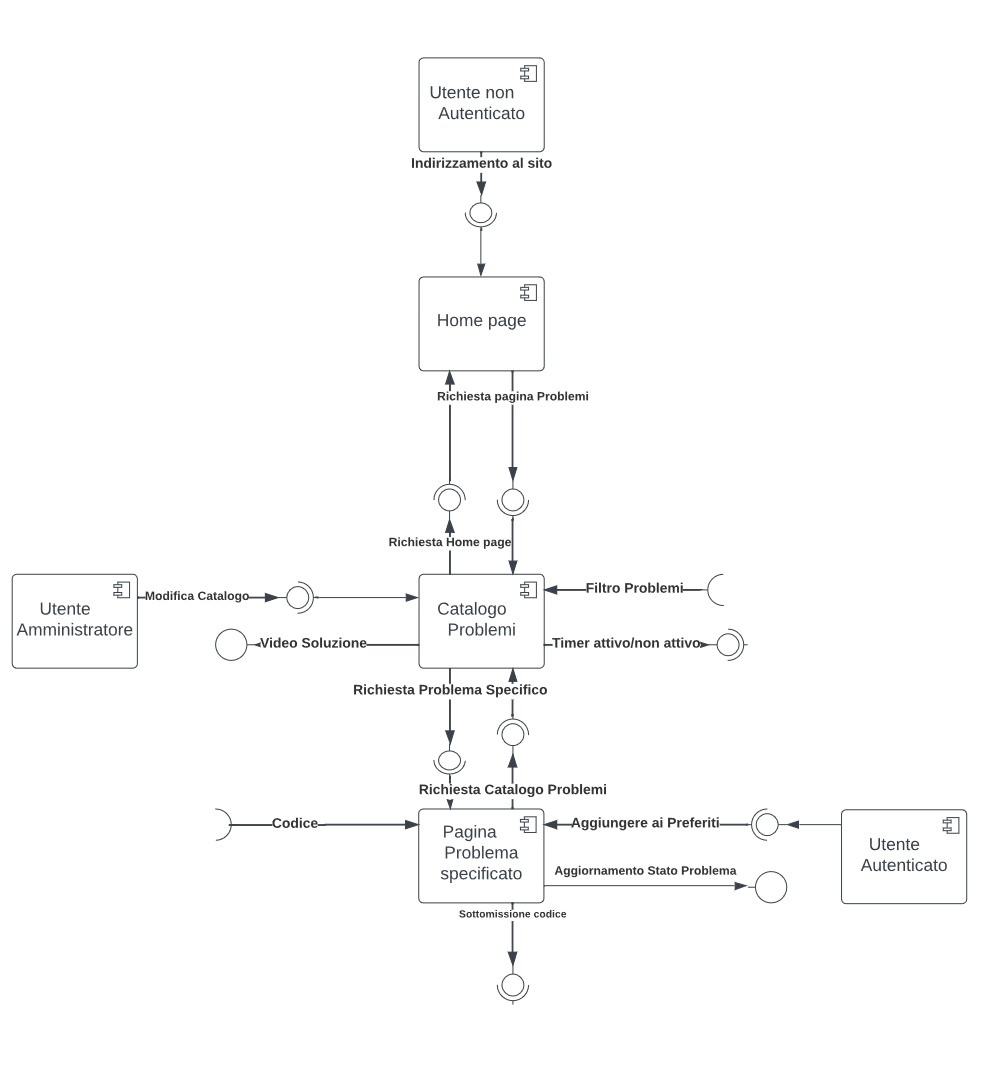
\includegraphics[width=1.2\textwidth]{materiale/site-ux.jpg}
%\end{center}
  
%\begin{center}
%    \hspace*{-1cm}
%    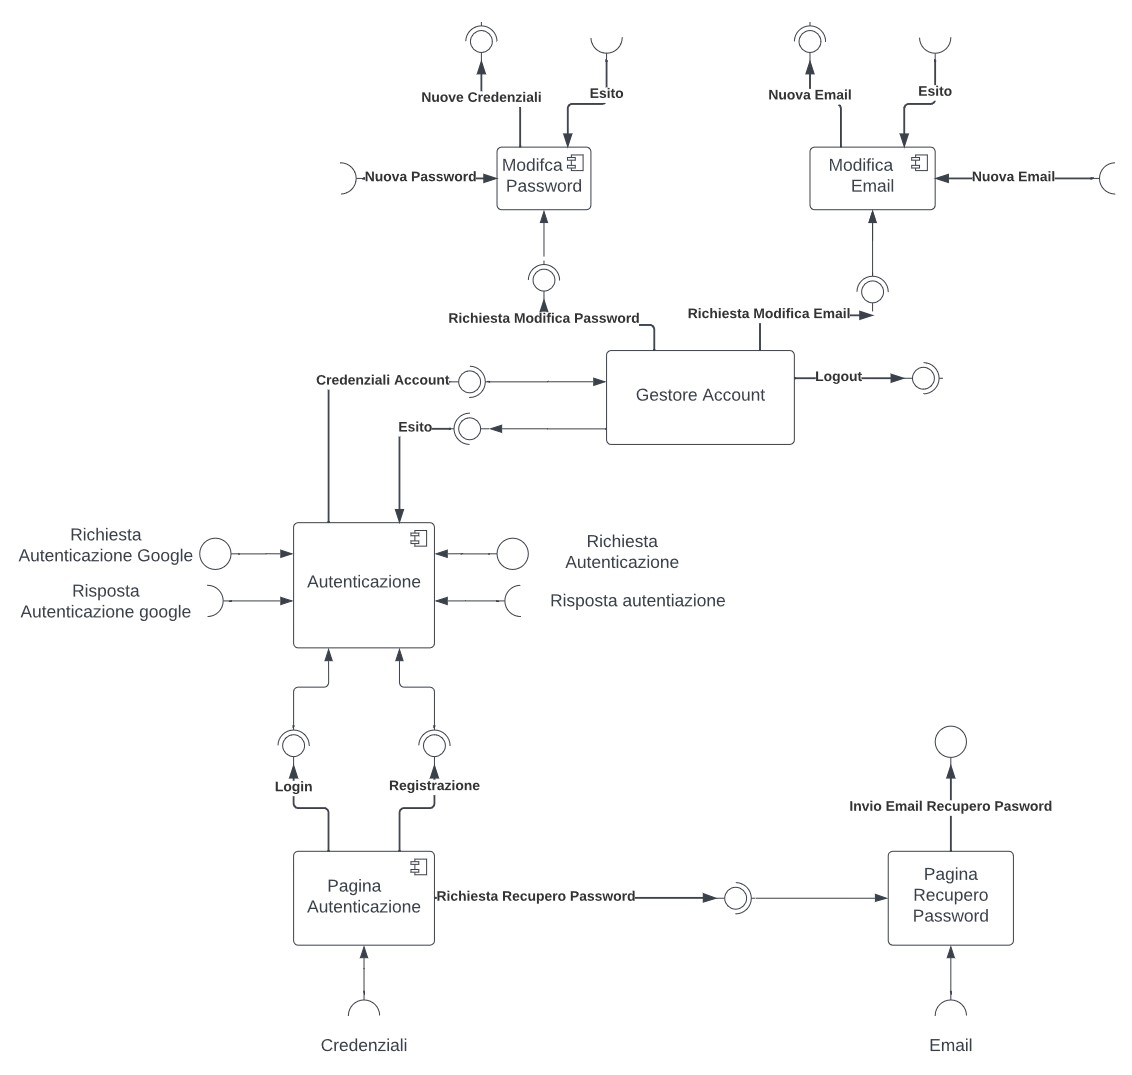
\includegraphics[width=1.2\textwidth]{materiale/login-component.jpg}
%\end{center}
    
\begin{figure}[H]
\centering
%\includegraphics[]{}
\caption{Diagramma dei Componenti}
\label{compdiagram}
\end{figure}
    


\end{document}